% Copyright 2015-2016 Dan Foreman-Mackey and the co-authors listed below.

\documentclass[manuscript, letterpaper]{aastex6}

\pdfoutput=1

\include{vc}

\usepackage{microtype}

\usepackage{url}
\usepackage{amssymb,amsmath}
\usepackage{natbib}
\bibliographystyle{aasjournal}

% ----------------------------------- %
% start of AASTeX mods by DWH and DFM %
% ----------------------------------- %

\setlength{\voffset}{0in}
\setlength{\hoffset}{0in}
\setlength{\textwidth}{6.5in}
\setlength{\textheight}{9in}
\setlength{\headheight}{0ex}
\setlength{\headsep}{\baselinestretch\baselineskip} % this is 2 lines in ``manuscript''
\setlength{\topmargin}{-\headsep}

\linespread{0.54} % close to 10/13 spacing in ``manuscript''
\setlength{\parindent}{0.54\baselineskip}
\hypersetup{colorlinks = false}
\makeatletter % you know you are living your life wrong when you need to do this
\long\def\frontmatter@title@above{
\vspace*{-\headsep}\vspace*{\headheight}
\noindent\footnotesize
{\noindent\footnotesize\textsc{\@journalinfo}}\par
{\noindent\scriptsize Preprint typeset using \LaTeX\ style AASTeX6 with
modifications by David W. Hogg and Daniel Foreman-Mackey.
}\par\vspace*{-\baselineskip}\vspace*{0.625in}
}%
\makeatother

% Section spacing:
\makeatletter
\let\origsection\section
\renewcommand\section{\@ifstar{\starsection}{\nostarsection}}
\newcommand\nostarsection[1]{\sectionprelude\origsection{#1}}
\newcommand\starsection[1]{\sectionprelude\origsection*{#1}}
\newcommand\sectionprelude{\vspace{1em}}
\makeatother

\sloppy\sloppypar

% ------------------ %
% end of AASTeX mods %
% ------------------ %

% Projects:
\newcommand{\project}[1]{\textsl{#1}}
\newcommand{\kepler}{\project{Kepler}}
\newcommand{\KT}{\project{K2}}
\newcommand{\tess}{\project{TESS}}
\newcommand{\pdc}{\project{PDC}}
\newcommand{\bls}{\project{BLS}}

\newcommand{\foreign}[1]{\emph{#1}}
\newcommand{\etal}{\foreign{et\,al.}}
\newcommand{\etc}{\foreign{etc.}}
\newcommand{\True}{\foreign{True}}
\newcommand{\Truth}{\foreign{Truth}}

\newcommand{\dfmfigref}[1]{\ref{fig:#1}}
\newcommand{\dfmFig}[1]{Figure~\dfmfigref{#1}}
\newcommand{\dfmfig}[1]{\dfmFig{#1}}
\newcommand{\dfmfiglabel}[1]{\label{fig:#1}}

% \newcommand{\Tab}[1]{Table~\ref{tab:#1}}
% \newcommand{\tab}[1]{\Tab{#1}}
\newcommand{\tablabel}[1]{\label{tab:#1}}

\renewcommand{\eqref}[1]{\ref{eq:#1}}
\newcommand{\Eq}[1]{Equation~(\eqref{#1})}
\newcommand{\eq}[1]{\Eq{#1}}
\newcommand{\eqalt}[1]{Equation~\eqref{#1}}
\newcommand{\eqlabel}[1]{\label{eq:#1}}

\newcommand{\sectionname}{Section}
\newcommand{\sectref}[1]{\ref{sect:#1}}
\newcommand{\Sect}[1]{\sectionname~\sectref{#1}}
\newcommand{\sect}[1]{\Sect{#1}}
\newcommand{\sectalt}[1]{\sectref{#1}}
\newcommand{\App}[1]{Appendix~\sectref{#1}}
\newcommand{\app}[1]{\App{#1}}
\newcommand{\sectlabel}[1]{\label{sect:#1}}

\newcommand{\T}{\ensuremath{\mathrm{T}}}
\newcommand{\dd}{\ensuremath{\,\mathrm{d}}}
\newcommand{\unit}[1]{{\ensuremath{\,\mathrm{#1}}}}
\newcommand{\bvec}[1]{{\ensuremath{\boldsymbol{#1}}}}
\newcommand{\appropto}{\mathrel{\vcenter{
  \offinterlineskip\halign{\hfil$##$\cr
    \propto\cr\noalign{\kern2pt}\sim\cr\noalign{\kern-2pt}}}}}
\newcommand{\densityunit}{{\ensuremath{\mathrm{nat}^{-2}}}}


% TO DOS
\newcommand{\todo}[3]{{\color{#2}\emph{#1}: #3}}
\newcommand{\dfmtodo}[1]{\todo{DFM}{red}{#1}}
\newcommand{\hoggtodo}[1]{\todo{HOGG}{blue}{#1}}


% Helpers for this paper:
\newcommand{\license}{MIT License}
\newcommand{\paper}{paper}

% Notation for this paper:
\newcommand{\meanpars}{{\ensuremath{\bvec{\theta}}}}
\newcommand{\kernpars}{{\ensuremath{\bvec{\alpha}}}}
\newcommand{\params}{{\ensuremath{\bvec{w}}}}
\newcommand{\poppars}{{\ensuremath{\bvec{\beta}}}}
\newcommand{\rate}{{\ensuremath{\Gamma}}}

\newcommand{\modelname}[1]{{\textsf{#1}}}


\shorttitle{The population of long-period exoplanets}
\shortauthors{Foreman-Mackey, Hogg, Morton, \etal}
% \submitted{Submitted to \textit{The Astrophysical Journal}}

\begin{document}

\title{%
The population of long-period exoplanets --- \\
Fully-automated discovery \& characterization of
long-period transiting exoplanet candidates in the \kepler\ archive
\vspace{-3\baselineskip}  % OMG AASTEX6 IS SO BROKEN
}

\newcounter{affilcounter}
\setcounter{affilcounter}{2}
\altaffiltext{1}{\url{danfm@uw.edu}; Sagan Fellow}

\edef \uw {\arabic{affilcounter}}\stepcounter{affilcounter}
\altaffiltext{\uw}       {Astronomy Department, University of Washington,
                          Seattle, WA, 98195, USA}

\edef \scda {\arabic{affilcounter}}\stepcounter{affilcounter}
\altaffiltext{\scda}     {Simons Center for Data Analysis, 160 Fifth Avenue,
                          7th floor, New York, NY 10010, USA}

\edef \nyu       {\arabic{affilcounter}}\stepcounter{affilcounter}
\altaffiltext{\nyu}      {Center for Cosmology and Particle Physics,
                          New York University,
                          4 Washington Place, New York, NY, 10003, USA}

\edef \cds       {\arabic{affilcounter}}\stepcounter{affilcounter}
\altaffiltext{\cds}      {Center for Data Science, New York University,
                          726 Broadway, 7th Floor, New York, NY, 10003, USA}

\edef \mpia      {\arabic{affilcounter}}\stepcounter{affilcounter}
\altaffiltext{\mpia}     {Max-Planck-Institut f\"ur Astronomie,
                          K\"onigstuhl 17, D-69117 Heidelberg, Germany}

\edef \princeton {\arabic{affilcounter}}\stepcounter{affilcounter}
\altaffiltext{\princeton}{Department of Astrophysics, Princeton University,
                          Princeton, NJ, 08544, USA}

\edef \mpis      {\arabic{affilcounter}}\stepcounter{affilcounter}
\altaffiltext{\mpis}     {Max Planck Institute for Intelligent Systems
                          Spemannstrasse 38, 72076 T\"ubingen, Germany}

\author{%
    Daniel~Foreman-Mackey\altaffilmark{1,\uw},
    David~W.~Hogg\altaffilmark{\scda,\nyu,\mpia,\cds},
    Timothy~D.~Morton\altaffilmark{\princeton},
    Bernhard~Sch\"olkopf\altaffilmark{\mpis},
    Eric~Agol\altaffilmark{\uw},
    and others
}



\begin{abstract}

The \kepler\ Mission has discovered thousands of exoplanets and revolutionized
our understanding of their population.
This large, homogeneous catalog of discoveries has enabled rigorous studies of
the occurrence rate of exoplanets and extra-Solar planetary systems as a
function of their physical properties.
Transit survey like \kepler\ are most sensitive to planets with shorter
orbital periods than the gas giant planets that dominate the dynamics of our
Solar System.
We performed a fully-automated search for the transits of long-period
exoplanets in the archival \kepler\ light curves and announce XXX planet
candidates.
Since our method involves no human intervention, we empirically characterize
the completeness and reliability of our search.
Based on these results, we measure the average occurrence rate of exoplanets
smaller than Jupiter and with orbital periods longer than 700 days to be $\dd
N = YYY \pm ZZZ\dd \ln P \dd \ln R$.

\end{abstract}

\keywords{%
methods: data analysis
---
methods: statistical
---
catalogs
---
planetary systems
---
stars: statistics
}

\section{Introduction}

EB catalog: \citep{Kirk:2016}

Microlensing OR: \citep{Shvartzvald:2016}

Data from the \kepler\ Mission has been used to discover thousands of
transiting exoplanets.
The systematic nature of these discoveries and careful quantification of
survey selection effects, search completeness, and catalog reliability has
enabled many diverse studies of the detailed frequency and distribution of
exoplanets \citep[for example,][]{Howard:2012, Petigura:2013,
Foreman-Mackey:2014, Dressing:2015, Burke:2015, Mulders:2015}.
So far, these results have been limited to relatively short orbital periods
because existing transit search methods require the observation of multiple
transits within the baseline of the data.
For \kepler, with a baseline of about four years, this sets an absolute upper
limit on the detectable periods of about two years.
In the Solar System, Jupiter~--~with a period of 12 years~--~dominates the
planetary dynamics and, since it would only exhibit at most one transit in the
\kepler\ data, an exo-Jupiter would be missed by most existing transit search
procedures.
It is possible to discover long-period planets like this using targeted radial
velocity (RV) surveys \citep[for example][]{Butler:2006, Knutson:2014,
Bryan:2016} but the cost of implementing a systematic RV search is
substantially higher than searching the existing and forthcoming photometric
data for single transits.

There are two main technical barriers to a systematic search for single
transit events.
The first is that the transit probability for long-period planets is very low;
scaling as $\propto P^{-5/3}$ for orbital periods longer than the
baseline of contiguous observations.
Therefore, even if long-period planets are intrinsically common, they will
be underrepresented in a transiting sample.
The second challenge is that there are many signals in the observed light
curves caused by stochastic processes~--~both instrumental and
astrophysical~--~that can masquerade as transits.
Even when the most sophisticated methods for removing this variability are
used, false signals far outnumber the true single transits in any traditional
search.

At the heart of all periodic transit search procedures is a filtering step
based on ``box least squares'' \citep[\bls;][]{Kovacs:2002}.
This step produces a list of candidate transit times that is then vetted to
remove the substantial fraction of false signals using some combination of
automated heuristics and expert curation.
In practice, the fraction of false signals can be substantially reduced by
requiring that at least three self-consistent transits be observed
\citep{Petigura:2013, Burke:2014, Rowe:2015, Coughlin:2016}.

Recent work has yielded discoveries of long-period transiting planets with
only one or two transits identified in archival \kepler\ and \KT\ light curves
by visual inspection \citep{Wang:2013, Kipping:2014a, Osborn:2016,
Kipping:2016, Uehara:2016, Wang:2015}.
Since all of these discoveries rely on human interaction, it is intractable to
reliably constrain the completeness of these catalogs and they cannot be used
to measure the occurrence rate of long-period planets.

In this \paper, we develop a systematic method of reliably discovering the
transits of large long-period companions in photometric time series
\emph{without human intervention}.
Since the search methodology is fully-automated, we can robustly measure the
search completeness~--~using injection and recovery tests~--~and use these
products to place probabilistic constraints on the occurrence rate of
long-period planets.
We apply this method to a subset of the archival data from the \kepler\
Mission and produce a catalog of discoveries.


\section{A fully-automated search method}

To find long-period exoplanets in the \kepler\ light curves, we search for
individual, high signal-to-noise transit signals using a fully-automated
procedure that can be broken into three main steps:
\begin{enumerate}
{\item an initial candidate search using a box-shaped matched filter,}
{\item light curve-level vetting (using automated model comparison) to remove
signals that don't match a transit shape, and}
{\item pixel-level vetting to remove some astrophysical false positives.}
\end{enumerate}
The following sections describe each of these steps in more detail.

The model comparison step (step 2) is the key component of our method that
enables robust automation but it is also computationally expensive because we
must estimate the marginalized likelihoods for the light curve under several
different models describing a transit and many other processes that ``look''
like transits but are actually caused by noise.
This step is also conservative; unless a signal is a very convincing transit,
it won't pass the test.
In practice, this means that all but the highest signal-to-noise events will
be rejected at this step.
Therefore, in the inexpensive first step~--~the initial candidate search~--~we
can restrict the candidate list to high signal-to-noise events without a
substantial loss in detection efficiency.

\subsection{Step 1 -- Initial candidate events}

It is not computationally feasible to run a full model comparison at every
time in the light curve so we must first find potentially interesting events.
For our purposes, ``interesting'' means high signal-to-noise and previously
unknown.

To generate this list, we use a method much like the standard ``box least
squares'' (BLS; \dfmtodo{CITE}) procedure with a single (non-periodic) box.
First, we filter the PDC (\dfmtodo{CITE}) light curves using a running
windowed median with a half-width of \dfmtodo{how many} to remove stellar
variability.
We then compute the signal-to-noise of the depth of a 0.6~day long
transit on a grid of times spanning the full baseline of observations.

In detail, at each proposal time $t_0$, we hypothesize a box-shaped transit
with duration $\tau$
\begin{eqnarray}
m(t) &=& \left\{\begin{array}{ll}
    \mu, & \mbox{\,if $|t - t_0| < \tau/2$} \\
    \mu - \delta, & \mbox{\,otherwise}
\end{array}\right. \quad.
\end{eqnarray}
Assuming that the uncertainties on the observed fluxes $f(t)$ are Gaussian
with known variance ${\sigma_f}^2$, the likelihood function for the mean flux
$\mu$ and transit depth $\delta$ can be analytically computed to be a
two-dimensional Gaussian with mean and covariance given by linear
least-squares.
This likelihood function provides a natural scalar objective: the
signal-to-noise of the measured depth $\delta / \sigma_\delta$ computed a
function of time.
In principle this scalar is also a function of duration but we only use a
single transit duration because the following steps in this procedure are only
sensitive to transits with very high signal-to-noise.
In practice, the final results are insensitive to the specific choice of
duration.

To avoid edge effects, we apodize this detection scalar near any large gaps in
the time series using a logistic function with width equal to one transit
duration.
Finally, we estimate the background noise level in the detection scalar time
series using a robust running windowed variance estimate of the detection
scalar and accepting peaks more than 25-times this noise as candidates.

For the \kepler\ light curves, this procedure yields at least one candidate
event in about 1~percent of targets and the three highest signal-to-noise
events are investigated in the following step.

\subsection{Step 2 -- Light curve vetting}

In this step of the method, the goal is to discard any signals that are not
sufficiently ``transit-like'' in shape.
To quantify this decision, we perform a model comparison between a physical
transit model and a set of other parameterized models for systematics.
In order for a candidate to pass this vetting step, the transit model must be
``preferred'' to any other model as measured using the Bayesian Information
Criterion (BIC).
The BIC is not the optimal choice for this model comparison but it is
computationally intractable to compute thousands of precise marginalized
likelihoods for each model.
The BIC can be efficiently computed and it exhibits the desired
behavior~--~increasing with the likelihood but flexible models are
penalized~--~and we find that it performs sufficiently well in practice.

For up to three candidate transit times per light curve, we select a
contiguous chunk of PDC light curve approximately centered on the proposed
transit with no more than 500 cadences \dfmtodo{check me} and compute the BIC
of each model for this data set.
The BIC for a model $k$ in the set of $K$ models is given by
\begin{eqnarray}
\mathrm{BIC}_k &=& \ln \mathcal{L}^* - \frac{J}{2}\,\log N
\end{eqnarray}
where the likelihood function $\mathcal{L}$ is evaluated at its maximum, $J$
is the number of free parameters in the model, and $N$ is the number of
data points in the data set.

For each model, we describe the data using a Gaussian Process (GP;
\dfmtodo{cite}) with a Mat\'ern-3/2 covariance and mean given by the chosen
model $m_k(t;\,\meanpars)$ parameterized by the parameter vector \meanpars.

We consider the following mean models and this list provides a qualitative
justification for each model:
\begin{itemize}
{\item \modelname{transit} -- a limb-darkened, exposure time integrated
transit light curve,}
{\item \modelname{variability} -- a pure Gaussian Process model to capture
stellar variability,}
{\item \modelname{outlier} -- a single outlier to account for a bad data
point,}
{\item \modelname{step} -- a step function to describe sudden pixel
sensitivity dropouts (SPSDs; \dfmtodo{CITE}), and}
{\item \modelname{box} -- a box to catch signals that are well fit by the
search scalar but insufficiently transit-like to be convincing.}
\end{itemize}
The functional forms of these models are given in Appendix \dfmtodo{SOME APP}.

\dfmfig{model-comp} shows representative events that fall into different
classes and the corresponding maximum-likelihood model.
For each candidate event, the BIC of each of these models is computed and the
event is only passed as a candidate if the \modelname{transit} model is
preferred to all the other models.
The \modelname{box} model is the most restrictive comparison, vetoing about
half of the candidate events in the \kepler\ light curves, followed by the
\modelname{variability} model.
To further restrict to non-grazing transits, we also reject events where the
best fit impact parameter is less than $1 - R_\mathrm{P} / R_\star$.

The reliability of this method of automated vetting is limited by the specific
models selected in this step.
We find that these are sufficient for the targets discussed below but other
target lists might require additional models to be included for robust
selection.

\begin{figure*}[p]~\\
\begin{center}
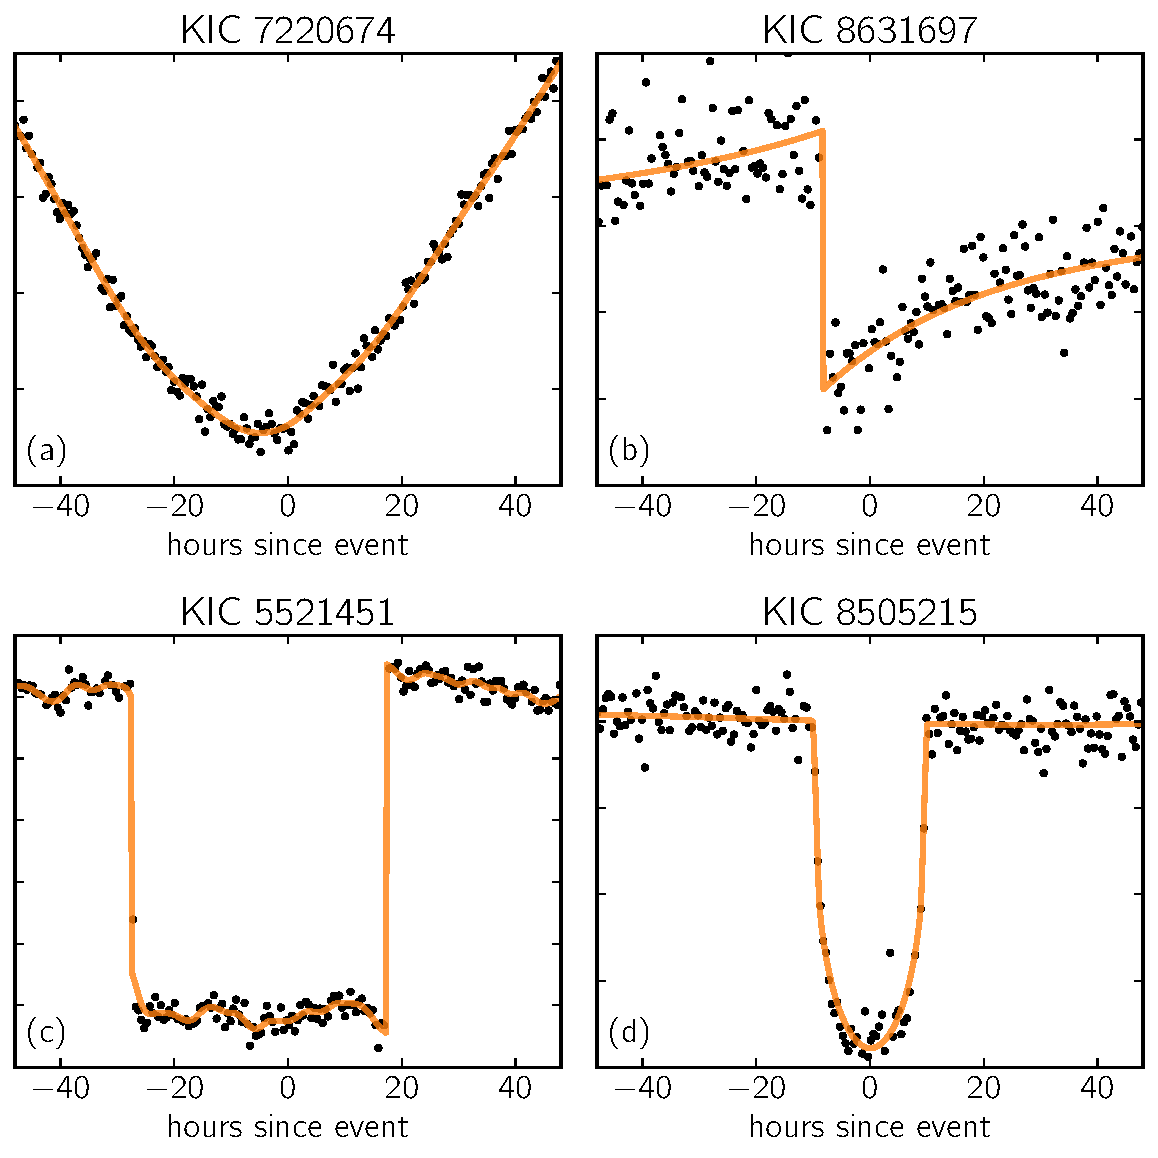
\includegraphics[width=\textwidth]{figures/model_comp.pdf}
\end{center}
\caption{%
Representative examples of candidate events flagged by the initial search.
Each example falls into a different model category and the figure shows the
data as black points and the best fit mean model prediction.
The examples represent the following model categories:
\emph{(a)} variability, \emph{(b)} step, \emph{(c)} box, and \emph{(d)}
transit.
\dfmfiglabel{model-comp}}
\end{figure*}


\subsection{Step 3 -- Pixel-level vetting}

To minimize contamination from background eclipsing binary systems, we require
candidate events to pass a centroid shift test similar to the one used in the
official \kepler\ transit search pipeline \citep{Bryson:2013}.
To measure the centroid shift, we model the flux-weighted centroid traces
independently in each coordinate as a multiple of the best-fit transit model
and a GP noise model.
By properly normalizing the transit model, we  measure the in-transit centroid
shift $\Delta_\mathrm{centroid}$ in pixels.
We reject any candidate event where the estimated transit location is more
than half a pixel from the out-of-transit centroid
\begin{eqnarray}
\Delta_\mathrm{centroid}\,\left(\frac{1}{\delta} - 1\right) &>& 0.5
\end{eqnarray}
where $\delta$ is the observed transit depth \citep{Bryson:2013}.


\section{Results: a catalog of long-period transiting exoplanet candidates}

To limit the scope of this paper while still demonstrating the applicability
of our method, we search the \kepler\ archival light curves of the brightest
and quietest Sun-like stars for long-period transiting exoplanets.
In this section, we describe the target selection process, the parameter
estimation procedure, and present the catalog of discoveries.


\subsection{Target selection}\sectlabel{target-selection}

We select the $\sim40,000$ brightest and quietest G and K dwarfs from the
\kepler\ catalog using the most recent catalog of stellar parameters%
\footnote{Parameters from the \textsf{q1\_q17\_dr24\_stellar} table from the
NASA Exoplanet Archive \citep[][with updates]{Huber:2014}.} and the cuts used
by \citet{Burke:2015}:
\begin{itemize}
{\item $4200\unit{K} \le T_\mathrm{eff} \le 6100\unit{K}$,}
{\item $R_\star \le 1.15\,R_\odot$,}
{\item $\mathrm{data\,span} \ge 2\,\mathrm{years}$,}
{\item $\mathrm{duty\,cycle} \ge 0.6$,}
{\item $K_p \le 15\unit{mag}$, and}
{\item $\mathrm{CDPP}_{7.5\unit{hrs}} \le 1000\unit{ppm}$.}
\end{itemize}
We continue by excluding the light curves of known eclipsing
binaries\footnote{\url{http://keplerebs.villanova.edu/}} \citep{Kirk:2016},
other known false positives \citep{Coughlin:2016}, a planet with known transit
timing variations (Kepler-9), and four especially noisy stars (KIC~4482348,
KIC~4450472, KIC~5438845, and KIC~10068041).
The final catalog contains 39,036 targets and the parameter distribution is
shown in \dfmfig{targets}.

Since these data have already been searched for short-period planets, we
assume that all high signal-to-noise candidates with three or more transits
have been previously found \citep{Coughlin:2016}.
To remove these candidates from consideration, we mask the cadences within two
transit durations of the time when a short-period planet candidate is known to
transit\footnote{We specifically use the \textsf{q1\_q17\_dr24\_koi} from the
NASA Exoplanet Archive \url{http://exoplanetarchive.ipac.caltech.edu/}.}.

\begin{figure}~\\
\begin{center}
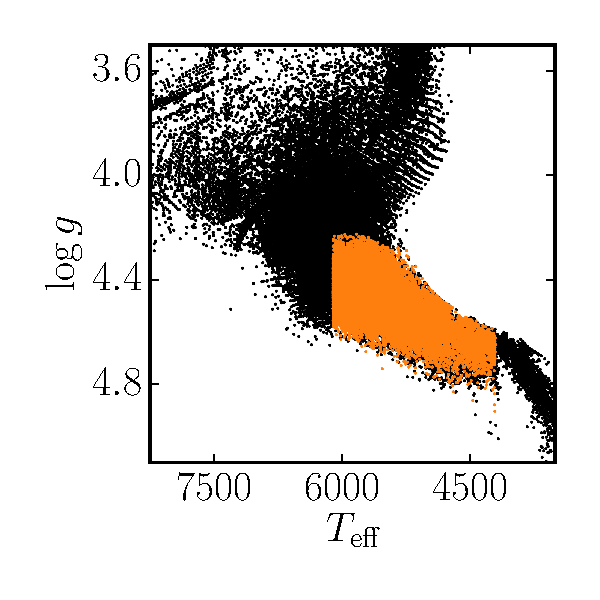
\includegraphics{figures/targets.pdf}
\end{center}
\caption{%
Blah.
\dfmfiglabel{targets}}~\\
\end{figure}


\subsection{Parameter estimation}

\begin{figure*}[p]~\\
\begin{center}
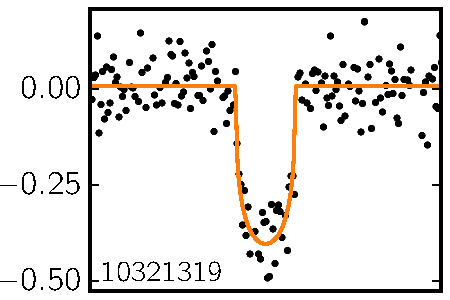
\includegraphics[width=0.24\textwidth]{figures/lcs/10321319.pdf}
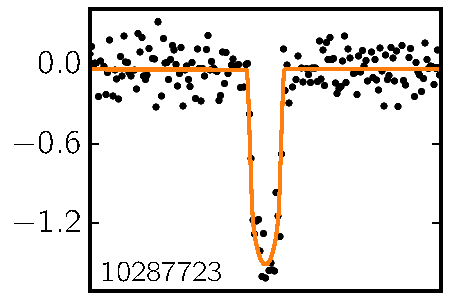
\includegraphics[width=0.24\textwidth]{figures/lcs/10287723.pdf}
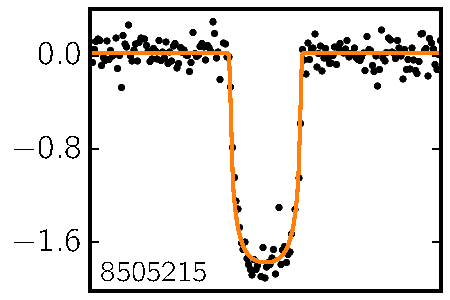
\includegraphics[width=0.24\textwidth]{figures/lcs/8505215.pdf}
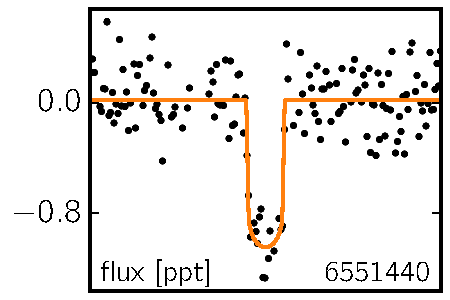
\includegraphics[width=0.24\textwidth]{figures/lcs/6551440.pdf}
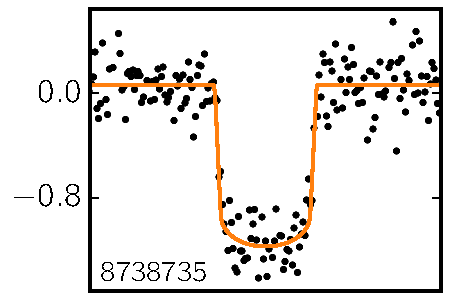
\includegraphics[width=0.24\textwidth]{figures/lcs/8738735.pdf}
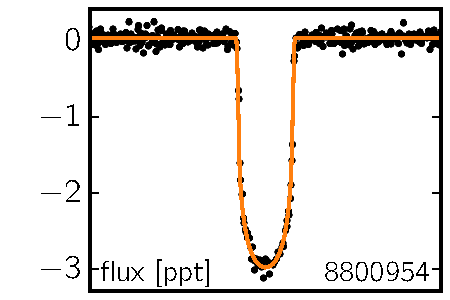
\includegraphics[width=0.24\textwidth]{figures/lcs/8800954.pdf}
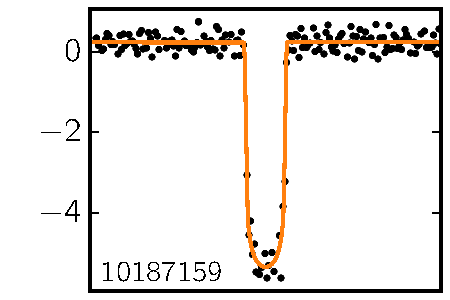
\includegraphics[width=0.24\textwidth]{figures/lcs/10187159.pdf}
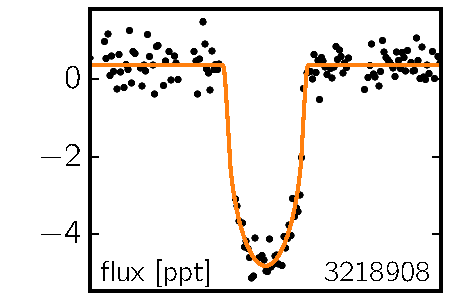
\includegraphics[width=0.24\textwidth]{figures/lcs/3218908.pdf}
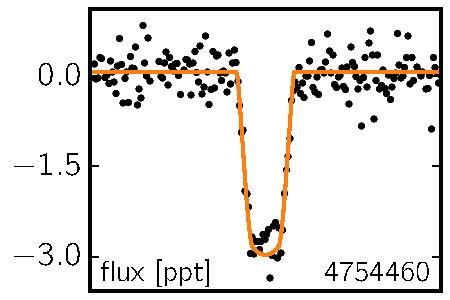
\includegraphics[width=0.24\textwidth]{figures/lcs/4754460.pdf}
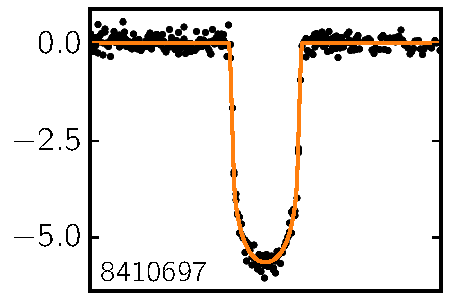
\includegraphics[width=0.24\textwidth]{figures/lcs/8410697.pdf}
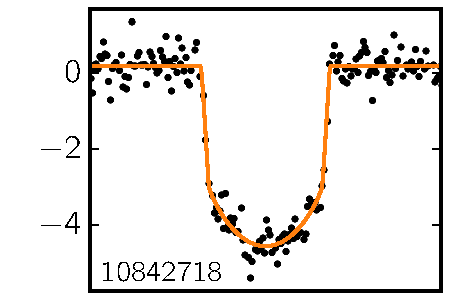
\includegraphics[width=0.24\textwidth]{figures/lcs/10842718.pdf}
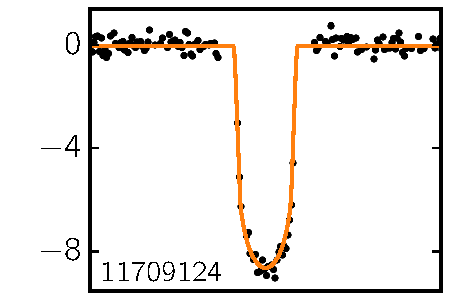
\includegraphics[width=0.24\textwidth]{figures/lcs/11709124.pdf}
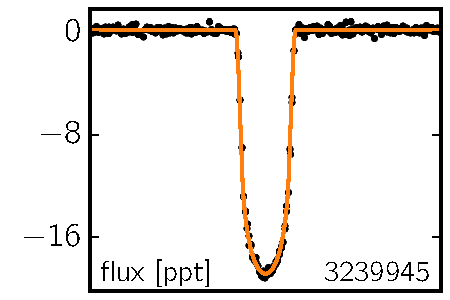
\includegraphics[width=0.24\textwidth]{figures/lcs/3239945.pdf}
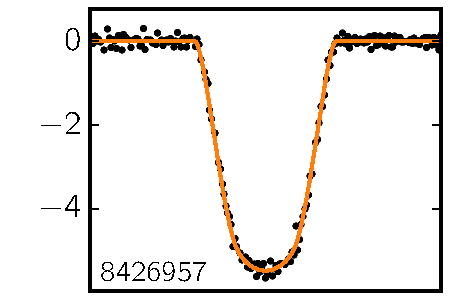
\includegraphics[width=0.24\textwidth]{figures/lcs/8426957.pdf}
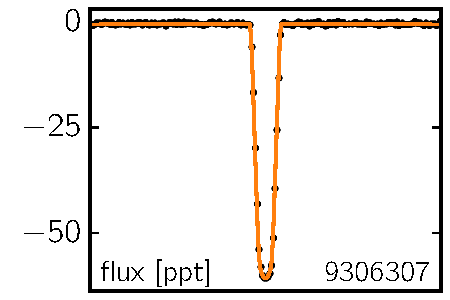
\includegraphics[width=0.24\textwidth]{figures/lcs/9306307.pdf}
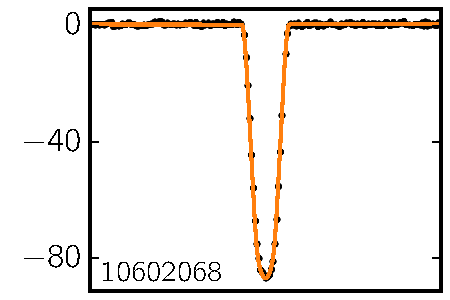
\includegraphics[width=0.24\textwidth]{figures/lcs/10602068.pdf}

\end{center}
\caption{%
\dfmfiglabel{lightcurves}}
\end{figure*}

\begin{figure*}~\\
\begin{center}
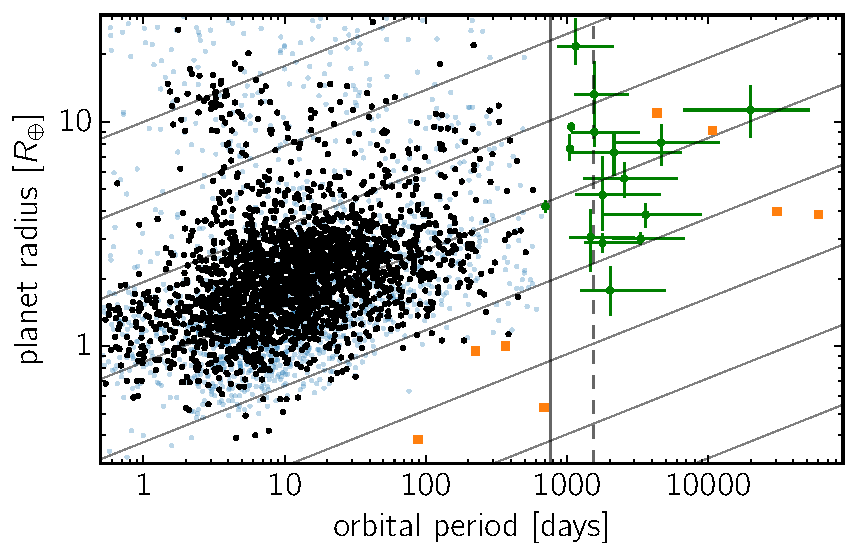
\includegraphics{figures/full_sample_plus_cands.pdf}
\end{center}
\caption{%
Blah.
\dfmfiglabel{full-sample}}~\\
\end{figure*}

\begin{deluxetable}{cccccl}
\tabletypesize{\footnotesize}
\tablecaption{caption\label{tab:table}}
\tablehead{
    \colhead{kic id} & \colhead{period [years]} & \colhead{$t_0$ [KBJD]} &
    \colhead{radius [$R_\mathrm{J}$]} & \colhead{$T_\mathrm{eq}$ [K]} &
    \colhead{comments}
}
\startdata
3218908 & $7.0_{-3.4}^{+9.5}$ & $766.6722_{-0.0114}^{+0.0096}$ & $0.514_{-0.093}^{+0.092}$ & $129_{-39}^{+41}$ & KOI 1108 / Kepler-770\\
3239945 & $2.9328721(26)$ & $420.28714_{-0.00068}^{+0.00069}$ & $0.876\pm0.039$ & $142.8_{-4.2}^{+4.3}$ & KOI 490 / Kepler-167\\
4754460 & $5.9_{-3.0}^{+11.8}$ & $826.8369\pm0.0046$ & $0.67_{-0.15}^{+0.16}$ & $171_{-64}^{+59}$ & \\
6551440 & $4.0_{-1.2}^{+4.2}$ & $1039.0589\pm0.0037$ & $0.282_{-0.083}^{+0.093}$ & $170_{-45}^{+38}$ & \\
8410697 & $2.8688097(54)$ & $542.1231\pm0.0013$ & $0.698_{-0.078}^{+0.107}$ & $206_{-13}^{+15}$ & \\
8426957 & $54_{-36}^{+88}$ & $784.677\pm0.013$ & $1.04_{-0.25}^{+0.30}$ & $85_{-28}^{+46}$ & \\
8505215 & $9.1_{-3.4}^{+9.5}$ & $140.0492_{-0.0018}^{+0.0017}$ & $0.277\pm0.017$ & $103_{-23}^{+19}$ & \\
8738735 & $9.9_{-5.0}^{+14.9}$ & $697.8538_{-0.0049}^{+0.0059}$ & $0.355_{-0.044}^{+0.045}$ & $136_{-39}^{+43}$ & KOI 693 / Kepler-214\\
8800954 & $1.9279957(91)$ & $492.7652\pm0.0024$ & $0.386\pm0.025$ & $189.4_{-7.3}^{+7.2}$ & KOI 1274 / Kepler-421\\
9306307 & $4.2_{-1.1}^{+3.2}$ & $1191.35648\pm0.00018$ & $1.20_{-0.33}^{+0.51}$ & $127\pm32$ & \\
10187159 & $4.9_{-1.8}^{+7.6}$ & $604.1102_{-0.0031}^{+0.0023}$ & $0.43_{-0.13}^{+0.21}$ & $119_{-43}^{+34}$ & KOI 1870 / Kepler-989\\
10287723 & $4.9_{-1.3}^{+4.3}$ & $393.5976_{-0.0029}^{+0.0031}$ & $0.266_{-0.024}^{+0.027}$ & $114_{-21}^{+13}$ & \\
10321319 & $5.5_{-2.1}^{+8.1}$ & $554.3562_{-0.0063}^{+0.0064}$ & $0.163_{-0.037}^{+0.046}$ & $153_{-47}^{+37}$ & \\
10602068 & $3.15_{-0.82}^{+2.79}$ & $830.80892\pm0.00015$ & $1.99_{-0.34}^{+0.66}$ & $158_{-34}^{+30}$ & \\
10842718 & $12.7_{-6.6}^{+20.2}$ & $226.2344\pm0.0047$ & $0.74\pm0.16$ & $128_{-43}^{+47}$ & \\
11709124 & $4.3_{-1.3}^{+4.7}$ & $657.2674_{-0.0016}^{+0.0018}$ & $0.83_{-0.11}^{+0.12}$ & $166_{-39}^{+28}$ & KOI 435 / Kepler-154\\
\enddata

% \tablenotetext{a}{Adjusted for inflation}
% \tablenotetext{b}{Accounts for the change from page charges to digital quanta in April, 2011}
% \tablecomments{Note that {\tt \string \colnumbers} does not work with the
% vertical line alignment token. If you want vertical lines in the headers you
% can not use this command at this time.}
\end{deluxetable}



\section{Empirical search completeness}

To measure the completeness of our long-period transit search method, we
exploit the fact that transit signals are sparse and rare.
Therefore, most light curves contain no transits and we can reliably measure
the recovery rate of our method on synthetic transit signals~--~with known
properties~--~injected into real light curves.
This procedure is standard practice in the transit literature and it has been
used to determine the completeness of the KOI catalog (\dfmtodo{cite}) and
other independent transit searches (\dfmtodo{cite}).

To reliably capture the full structure of the search completeness function,
the simulations must sample the (high-dimensional) space of all properties
that affect the probability of detecting a transit: the stellar properties
(including variability amplitudes and time scales), the planet's physical
properties and orbital elements, and any observational effects (noise,
spacecraft pointing variations, \etc).
For the modest goals of this paper, we only need a robust constraint on the
transit detection efficiency \emph{integrated} across the target sample but,
even so, many simulations per star are required.

The procedure for measuring the recovery rate of simulated transits is as
follows:
\begin{enumerate}
{\item First, a star is randomly selected from the target list, and the PDC
light curve and stellar properties for that star are loaded.}
{\item Planetary properties are sampled from the distributions listed in
\dfmtodo{some table} with phase uniformly distributed across the baseline of
observations. These properties are resampled until the transit is visible in
at least one non-flagged cadence.}
{\item The transit signal induced by this planet is computed and multiplied
into the PDC light curve.}
{\item The transit search method described in section \dfmtodo{some section}
(including de-trending and all automated vetting) is applied to this light
curve with the injected transit signal.}
{\item This candidate is flagged as recovered if at least one transit (within
\dfmtodo{some tolerance}) passes all the cuts imposed by the automated
vetting.}
\end{enumerate}

The fraction of recovered simulations as a function of the relevant parameters
gives an estimate of the search completeness or the probability of detecting
an exoplanet transit with a given set of parameters, \emph{conditioned on the
fact that it transits}.
We will call this function $Q_{\mathrm{det},k}(\params)$ where \params\ is the
set of all parameters affecting the transit detectability and $k$ is an index
running over target stars.

This detection efficiency must then be combined with the geometric transit
probability function and the window function.
For the star $k$, the geometric transit probability is given by \dfmtodo{cite}
\begin{eqnarray}
Q_{\mathrm{geom},k} (\params) &=& \frac{R_{\star,k}}{a_k}
    \, \frac{1 + e\,\sin\omega}{1-e^2} \\
&=& \left[\frac{4\,\pi^2}{G\,M_{\star,k}}\right]^{1/3}\,R_{\star,k}
    \, \left[\frac{1 + e\,\sin \omega}{1-e^2}\right]
    \, P^{-2/3}
\end{eqnarray}
where the parameters $e$, $\omega$, and $P$ are included in \params.
Approximating the window function using the binomial probability of observing
at least one transit \dfmtodo{cite bm14} we find
\begin{eqnarray}
Q_{\mathrm{win},k} (\params) &=& 1 - (1 - f_{\mathrm{duty},k})^{T_k/P}
\end{eqnarray}
where $f_{\mathrm{duty},k}$ is the duty cycle and $T_k$ is the full
observation baseline for target $k$.

Combining these detection effects, the total detection efficiency is given by
\begin{eqnarray}
Q_k(\params) &=& Q_{\mathrm{det},k}(\params) \,
                 Q_{\mathrm{win},k} (\params) \,
                 Q_{\mathrm{geom},k} (\params) \quad.
\end{eqnarray}
For the purposes of this \paper, we are not considering the occurrence rate of
exoplanets as a function of stellar properties; we will only measure an
average rate across the target sample that we previously selected.
Therefore, it is sufficient to estimate the marginalized detection efficiency
integrated with respect to our prior distributions on the nuisance parameters.
In this case, the only parameters that we will consider are planet radius and
orbital period.
Under this model, the relevant detection efficiency function for long-period
transiting planets is
\begin{eqnarray}\eqlabel{full-comp}
Q(R,\,P) &=& \frac{1}{K} \sum_{k=1}^{K} \int Q_k(\params) \,
    p(\params_{\{R,\,P\}}) \dd\params_{\{R,\,P\}}
\end{eqnarray}
where $\params_{\{R,\,P\}}$ indicates the set of all parameters except radius
and period.

Since the simulated parameters in the injection and recovery tests described
above were sampled from the prior distribution $p(\params_{\{R,\,P\}})$, the
easiest way to estimate \eq{full-comp} is to take the ratio of the weighted
histogram of the recovered injections to the weighted histogram of all
simulations where each simulation is weighted by
$Q_{\mathrm{win},k} (\params) \, Q_{\mathrm{geom},k} (\params)$ evaluated at
the parameters of the simulation.
\dfmtodo{Some figure} shows the measured completeness (\eq{full-comp}) as a
function of planet radius and orbital period.

\dfmtodo{Analytic fit?}

\begin{figure*}[p]~\\
\begin{center}
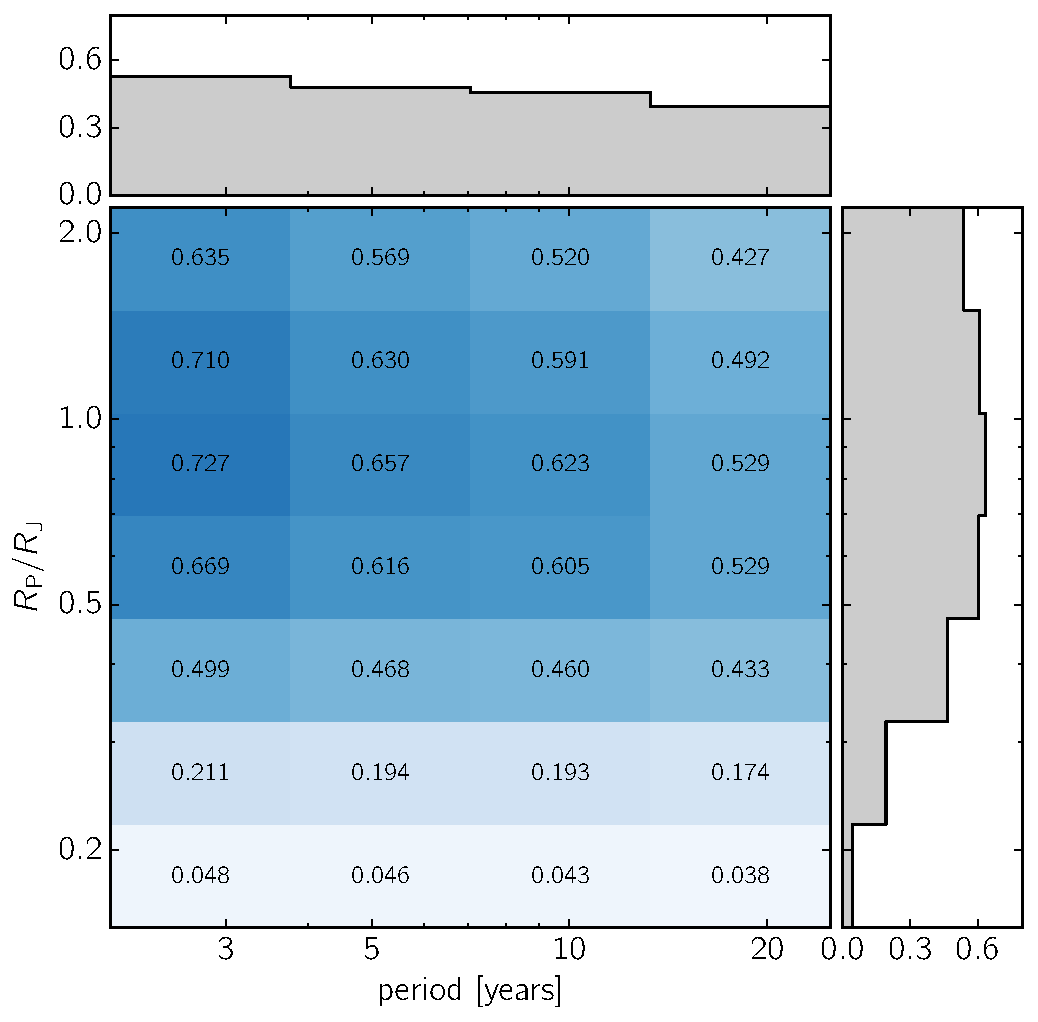
\includegraphics[width=\textwidth]{figures/completeness.pdf}
\end{center}
\caption{%
\dfmfiglabel{completeness}}
\end{figure*}


\section{The occurrence rate of long-period exoplanets}

Using the catalog of exoplanet discoveries (\dfmtodo{some section}) and the
measurement of the search completeness (\dfmtodo{some section}), we can now
estimate the occurrence rate of long-period exoplanets.
This inference can be simplified by making a few strong assumptions that are
only weakly justified.
First, we make the strong assumption that none of the candidates are
astrophysical false positives (background eclipsing binaries, the secondary
eclipse of a long-period binary system, \etc).
We revisit this assumption and discuss its validity in \dfmtodo{some section}.
Next, we model the occurrence of exoplanets as a Poisson process
(\dfmtodo{CITE}) with a rate function $\rate_{\poppars} (R,\,P)$ parameterized
by some parameters \poppars.
This assumption leads to the commonly used likelihood function
(\dfmtodo{CITE})
\begin{eqnarray}
\ln p (\{w_j\}_{j=1}^J\,|\,\poppars) =
    \sum_{j=1}^J \ln \rate_{\poppars} (R_j,\,P_j)
    - \int \rate_{\poppars} (R,\,P)\,Q(R,\,P)\dd R\dd P
    + \mathrm{constant} \quad.
\end{eqnarray}
Since our catalog of discoveries is small, we will only make limited
inferences about the population.
For the purposes of this paper, we will simply estimate the period of
long-period planets ($2\,\mathrm{yr} \le P < 15\,\mathrm{yr}$) in two radius
bins $0.1\,R_\mathrm{J} \le R < 0.5\,R_\mathrm{J}$ and $0.5\,R_\mathrm{J} \le
R < R_\mathrm{J}$.





\section{Astrophysical false positives}

Tim to write some words here.



\section{Discussion}\sectlabel{discussion}

We have developed a fully-automated method to search for the transits and
eclipses of long-period companions in photometric time series.
Applying this method to a subset of the \kepler\ archival light curves, we
discovered XX astrophysical transits.
Of these discoveries, at least about YY are likely to be planetary in nature.
Combining this catalog of discoveries with a measurement of the completeness
of our search method, we place a constraint on the occurrence rate of
long-period exoplanets.

Our method for transit detection finds convincing transit-shaped signals does
a model comparison between a physical transit model.

All of the code used in this project is available from
\url{https://github.com/dfm/peerless} under the MIT open-source software
license.
This code (plus some dependencies) can be run to re-generate all of the
figures and results in this \paper; this version of the paper was generated
with git commit \texttt{\githash} (\gitdate).


\acknowledgments
It is a pleasure to thank
\ldots
for helpful contributions to the ideas and code presented here.

DWH was partially supported by the National Science Foundation (grant
IIS-1124794), the National Aeronautics and Space Administration (grant
NNX12AI50G), and the Moore--Sloan Data Science Environment at NYU.

This research made use of the NASA \project{Astrophysics Data System} and the
NASA Exoplanet Archive.
The Exoplanet Archive is operated by the California Institute of Technology,
under contract with NASA under the Exoplanet Exploration Program.
This \paper\ includes data collected by the \kepler\ mission. Funding for the
\kepler\ mission is provided by the NASA Science Mission directorate.
We are grateful to the entire \kepler\ team, past and present.
Their tireless efforts were all essential to the tremendous success of the
mission and the successes of \KT, present and future.

These data were obtained from the Mikulski Archive for Space Telescopes
(MAST).
STScI is operated by the Association of Universities for Research in
Astronomy, Inc., under NASA contract NAS5-26555.
Support for MAST is provided by the NASA Office of Space Science via grant
NNX13AC07G and by other grants and contracts.

Computing resources were provided by High Performance Computing at New York
University.

\facility{Kepler}
\software{%
    \project{ceres} \citep{Agarwal:2016},
    \project{corner.py} \citep{Foreman-Mackey:2016},
    \project{emcee} \citep{Foreman-Mackey:2013},
    \project{george} \citep{Ambikasaran:2016},
	\project{matplotlib} \citep{Hunter:2007},
	\project{numpy} \citep{Van-Der-Walt:2011},
	\project{scipy} \citep{Jones:2001}}.

\newpage
\appendix

\section{Gaussian process regression}

Gaussian Processes (GPs) are a class of non-parametric, stochastic models that
have been demonstrated to be good effective models for the variability in
\kepler\ light curves.
A simple GP model can be used to capture residual non-transit variability in
light curves.
In this \paper, we use a GP model for two steps: light curve--level transit
shape vetting and parameter estimation.
A full discussion of GPs is beyond the scope of this \paper, so we will only
summarize the most relevant points here and direct an interested reader to
\dfmtodo{cite RW} for more details.

A GP model is specified by the following likelihood function
\begin{eqnarray}\eqlabel{gplike}
\mathcal{L} = \ln p(\bvec{y}\,|\,\meanpars,\,\kernpars) &=&
- \frac{1}{2}\,\bvec{r}(\meanpars)^\T\,K(\kernpars)^{-1}\,
    \bvec{r}(\meanpars)
- \frac{1}{2}\log\det K(\kernpars) - \frac{N}{2} \log{2\,\pi}
\end{eqnarray}
where \bvec{y} is a list of measurements in a scalar time series~--~in this
case, fluxes~--~measured at the times \bvec{t}, and
\begin{eqnarray}
\bvec{r}(\meanpars) &=& \bvec{y} - m(\bvec{t};\,\meanpars)
\end{eqnarray}
is the vector of residuals away from the mean model $m(\bvec{t};\,\meanpars)$.
For the purposes of this paper, we model the covariance matrix $K(\kernpars)$
using the Mat\'ern-3/2 kernel.
Under this model, the elements of $K(\kernpars)$ are given by
\begin{eqnarray}\eqlabel{matern}
\left[ K(\kernpars) \right]_{ij} &=& \sigma_i^2\,\delta_{ij}
    + \alpha^2 \left[ 1+\frac{|t_i - t_j|}{\sqrt{3}\,\tau} \right]
      \exp \left(-\frac{|t_i - t_j|}{\sqrt{3}\,\tau}\right)
\end{eqnarray}
where $\sigma_i$ is the reported uncertainty on the $i$-th measurement in the
time series and $\delta_{ij}$ is the Kronecker delta.

This covariance function (\eqalt{matern}) is specified by an amplitude
$\alpha$ and a time scale $\tau$ and we will simultaneously fit for these
hyperparameters $\kernpars=(\alpha,\,\tau)$ and the parameters of the mean
model \meanpars.
To efficiently find the parameter set that maximizes \eq{gplike} using a
non-linear optimization routine\footnote{We use the L-BFGS-B method as
implemented in SciPy \url{%
http://docs.scipy.org/doc/scipy/reference/generated/%
scipy.optimize.minimize.html}.},
it is useful to be able to compute the gradient of \eq{gplike} with respect to
the parameters \meanpars\ and \kernpars.
These gradients are given by
\begin{eqnarray}\eqlabel{gpmeangrad}
\frac{\dd\ln p(\bvec{y}\,|\,\meanpars,\,\kernpars)}{\dd \meanpars} &=&
\frac{\dd m(\bvec{t};\,\meanpars)}{\dd\meanpars}^\T \, K(\kernpars)^{-1} \,
    m(\bvec{t};\,\meanpars)
\end{eqnarray}
and
\begin{eqnarray}
\frac{\dd\ln p(\bvec{y}\,|\,\meanpars,\,\kernpars)}{\dd \kernpars} &=&
\frac{1}{2}\,\mathrm{Tr}\left(
    \left[ \bvec{\phi}\,\bvec{\phi}^\T - K(\kernpars)^{-1} \right]
    \,\frac{\dd K(\kernpars)}{\dd\kernpars}
\right)
\end{eqnarray}
where
\begin{eqnarray}
\bvec{\phi} &=& K(\kernpars)^{-1}\,\bvec{r}(\meanpars) \quad.
\end{eqnarray}

To evaluate \eq{gpmeangrad}, we must also evaluate the derivative of the mean
model with respect to its parameters.
For this \paper, the model $m(\bvec{t};\,\meanpars)$ will sometimes be the
limb-darkened, exposure time-integrated transit of a planet on a Keplerian
orbit and the parameters \meanpars\ are the physical and orbital parameters of
the planet and star.
Analytically computing the gradient of a simple transit model is possible
\citep{Pal:2008} but it becomes substantially more tedious as the model
becomes more realistic.
Therefore, we use a compile-time automatic differentiation library\footnote{%
More specifically, we use the \texttt{Jet} object from the BSD-licensed Ceres
Solver \url{http://ceres-solver.org}} \citep{Agarwal:2016} to compute first
derivatives of the full transit model to machine precision.


\clearpage
\bibliography{peerless}

\end{document}
